\section{Usability}

\subsection{Personas}

\subsection{Persona 1 - Alex Frei (Investigative Journalist)}

\subsubsection{Persona Overview}

\textbf{Name:} Alex Frei \\
\textbf{Age:} 32 \\
\textbf{Occupation:} Investigative Journalist \\
\textbf{Industry:} Media and News Reporting

\subsubsection{Background}
Alex is an experienced journalist specializing in political reporting.
Known for in-depth investigative pieces, Alex often covers high-stakes political events, requiring rapid access to historical web data for fact-checking.

\subsubsection{Goals}
\begin{itemize}
    \item Quickly archive web pages for timely reporting on political events.
    \item Maintain an archive of web pages for in-depth analysis and future reference.
    \item Retrieve archived URLs efficiently for referencing in articles and reports.
\end{itemize}

\subsubsection{Challenges}
\begin{itemize}
    \item Finding a tool that archives web pages instantly and reliably.
    \item Ensuring easy access and shareability of archived content.
    \item Managing a collection of archived URLs efficiently and effectively.
\end{itemize}

\subsubsection{Interactions with URL-Archiver}
\begin{itemize}
    \item Utilizes URL-Archiver's CLI for quick and efficient archiving.
    \item Values the open-source nature for trustworthiness in journalistic integrity.
    \item Relies on CSV output for organized referencing of archived content.
\end{itemize}

\subsection{Persona 2 - Dr. Emma Katrin Winter (Academic Researcher)}

\subsubsection{Persona Overview}

\textbf{Name:} Dr. Emma Katrin Winter \\
\textbf{Age:} 40 \\
\textbf{Occupation:} Academic Researcher \\
\textbf{Industry:} Higher Education

\subsubsection{Background}
Dr. Winter is a tenured professor focused on social sciences, often citing digital journals and data repositories.
She requires reliable digital archiving for scholarly citations and utilizes .bib files for managing bibliographic data.

\subsubsection{Goals}
\begin{itemize}
    \item Ensure accurate citation of web content in academic papers.
    \item Maintain and manage a digital archive of resources for teaching and research.
    \item Share archived content with academic peers for collaboration.
    \item Integrate archived URLs into .bib files for streamlined academic referencing.
\end{itemize}

\subsubsection{Challenges}
\begin{itemize}
    \item Needs a reliable method for archiving web pages.
    \item Seeks efficient integration of archived URLs into .bib files.
    \item Manages extensive digital archives for large-scale research projects.
\end{itemize}

\subsubsection{Interactions with URL-Archiver}
\begin{itemize}
    \item Uses URL-Archiver for capturing and archiving academic papers.
    \item Values the integration of archived URLs into .bib files for academic referencing.
    \item Relies on CSV file generation for organizing digital resources.
\end{itemize}

\subsection{Persona 3 - Michael Schwarz (Content Marketing Specialist)}

\subsubsection{Persona Overview}

\textbf{Name:} Michael Schwarz \\
\textbf{Age:} 35 \\
\textbf{Occupation:} Content Marketing Specialist \\
\textbf{Industry:} Digital Marketing

\subsubsection{Background}
Michael is a skilled content marketer, responsible for digital campaigns and web presence analytics in a dynamic marketing agency.
His role involves archiving web content for brand reputation management and competitive analysis.

\subsubsection{Goals}
\begin{itemize}
    \item Regularly archive web content for marketing audits and compliance.
    \item Manage a digital archive for campaign retrospectives.
    \item Ensure easy access to archived content for reviews and strategic planning.
\end{itemize}

\subsubsection{Challenges}
\begin{itemize}
    \item Needs a tool capable of archiving web content efficiently.
    \item Requires a streamlined process for accessing archived material.
    \item Seeks an archive system that is user-friendly and reliable.
\end{itemize}

\subsubsection{Interactions with URL-Archiver}
\begin{itemize}
    \item Regularly uses URL-Archiver for archiving online marketing content.
    \item Appreciates the CLI interface for ease and speed of use.
    \item Relies on the tool's capability to create organized audit trails.
\end{itemize}


\subsection{Storyboard}


\subsection{UX-Prototyping}
This section presents the initial version of our UX prototype for the URL-Archiver, created using Balsamiq.
The images below are a series of UI sketches that represent an early conceptualisation of the application's user experience.
This prototype does not reflect the current state of the application, but serves as an important step in our design process.
Each figure illustrates the key stages of user interaction, from starting the application to completing the archiving process.

\begin{figure}[h!]
    \centering
    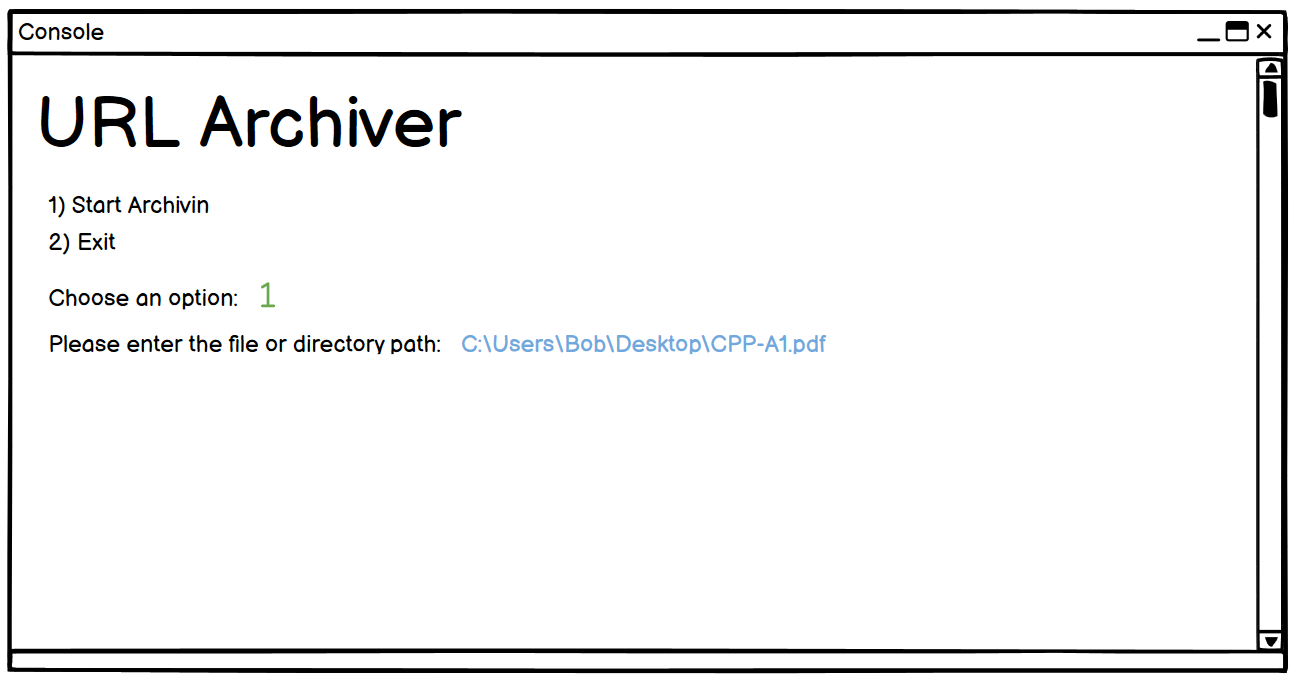
\includegraphics[width=1\textwidth]{pictures/UX-Prototype/Prototype_1}
    \caption{Starting point of the URL Archiver where the user is prompted to begin archiving or exit the application.}
    \label{fig:Initial_Interface}
\end{figure}
\begin{figure}[h!]
    \centering
    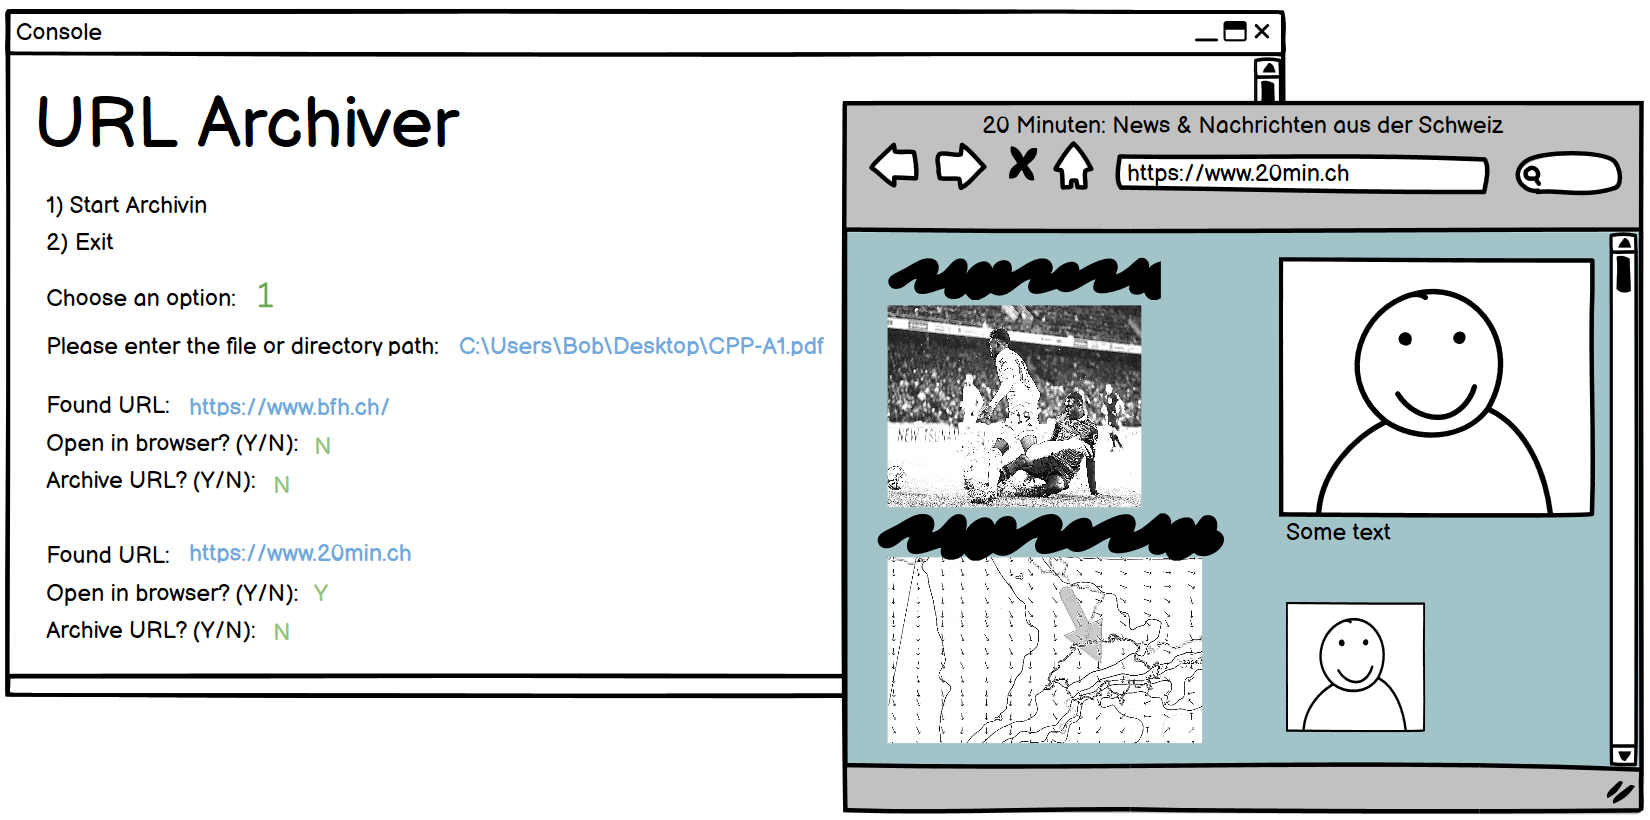
\includegraphics[width=1\textwidth]{pictures/UX-Prototype/Prototype_2}
    \caption{Upon choosing to open a URL in the browser, the user is presented with the live web page.}
    \label{fig:URL_Discovery}
\end{figure}
\begin{figure}[h!]
    \centering
    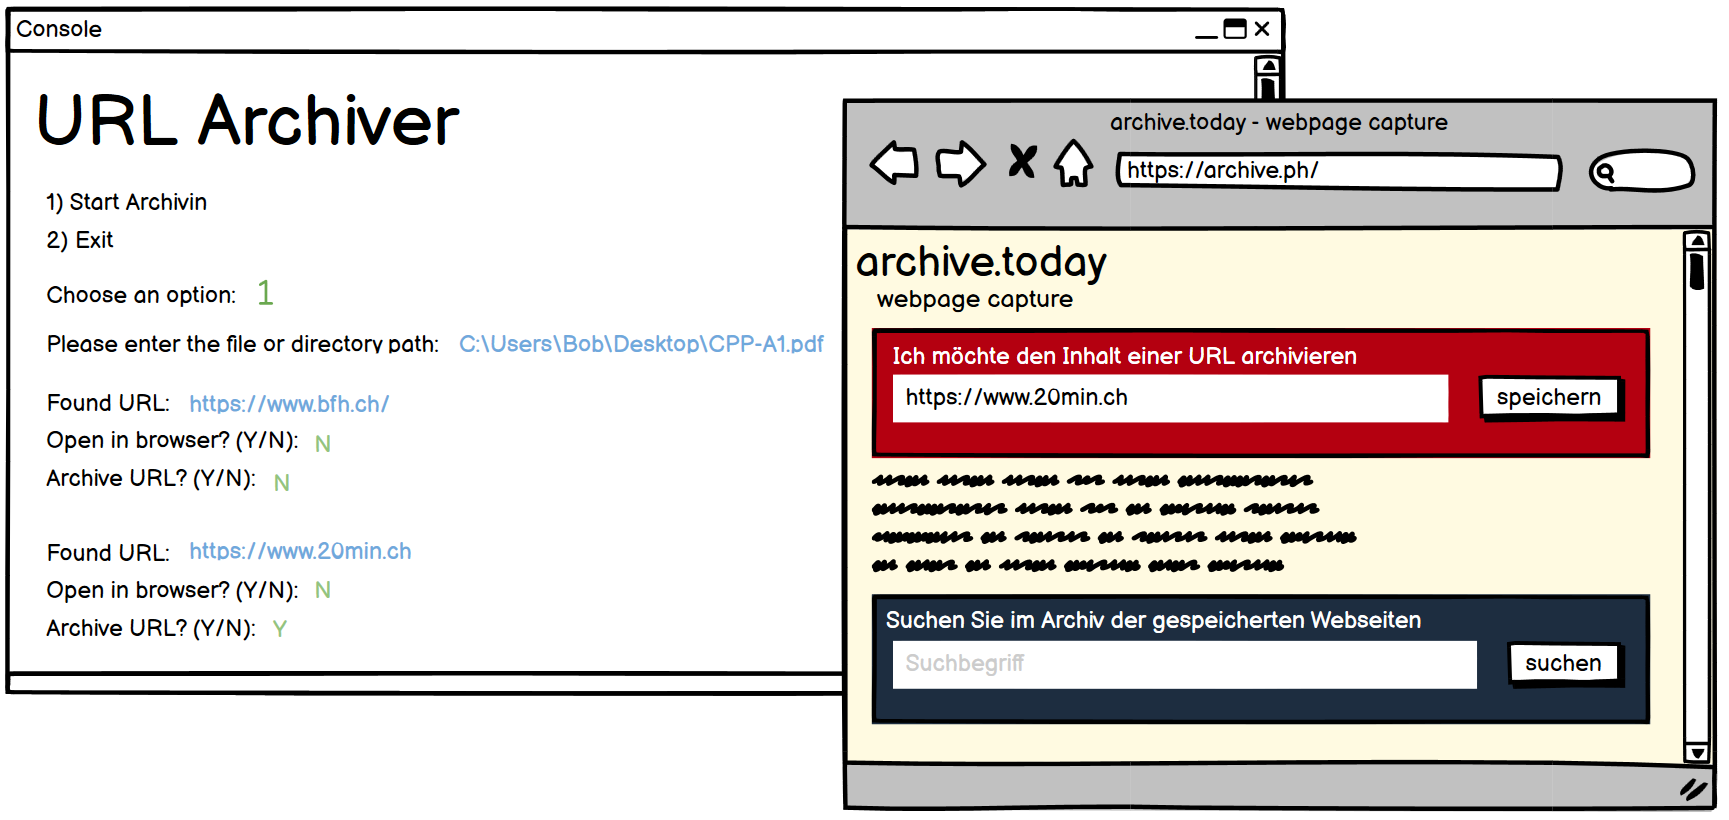
\includegraphics[width=1\textwidth]{pictures/UX-Prototype/Prototype_3}
    \caption{The user opts to archive the second URL, initiating the archiving process through the interface.}
    \label{fig:Browser_Interaction}
\end{figure}
\clearpage

\begin{figure}[h!]
    \centering
    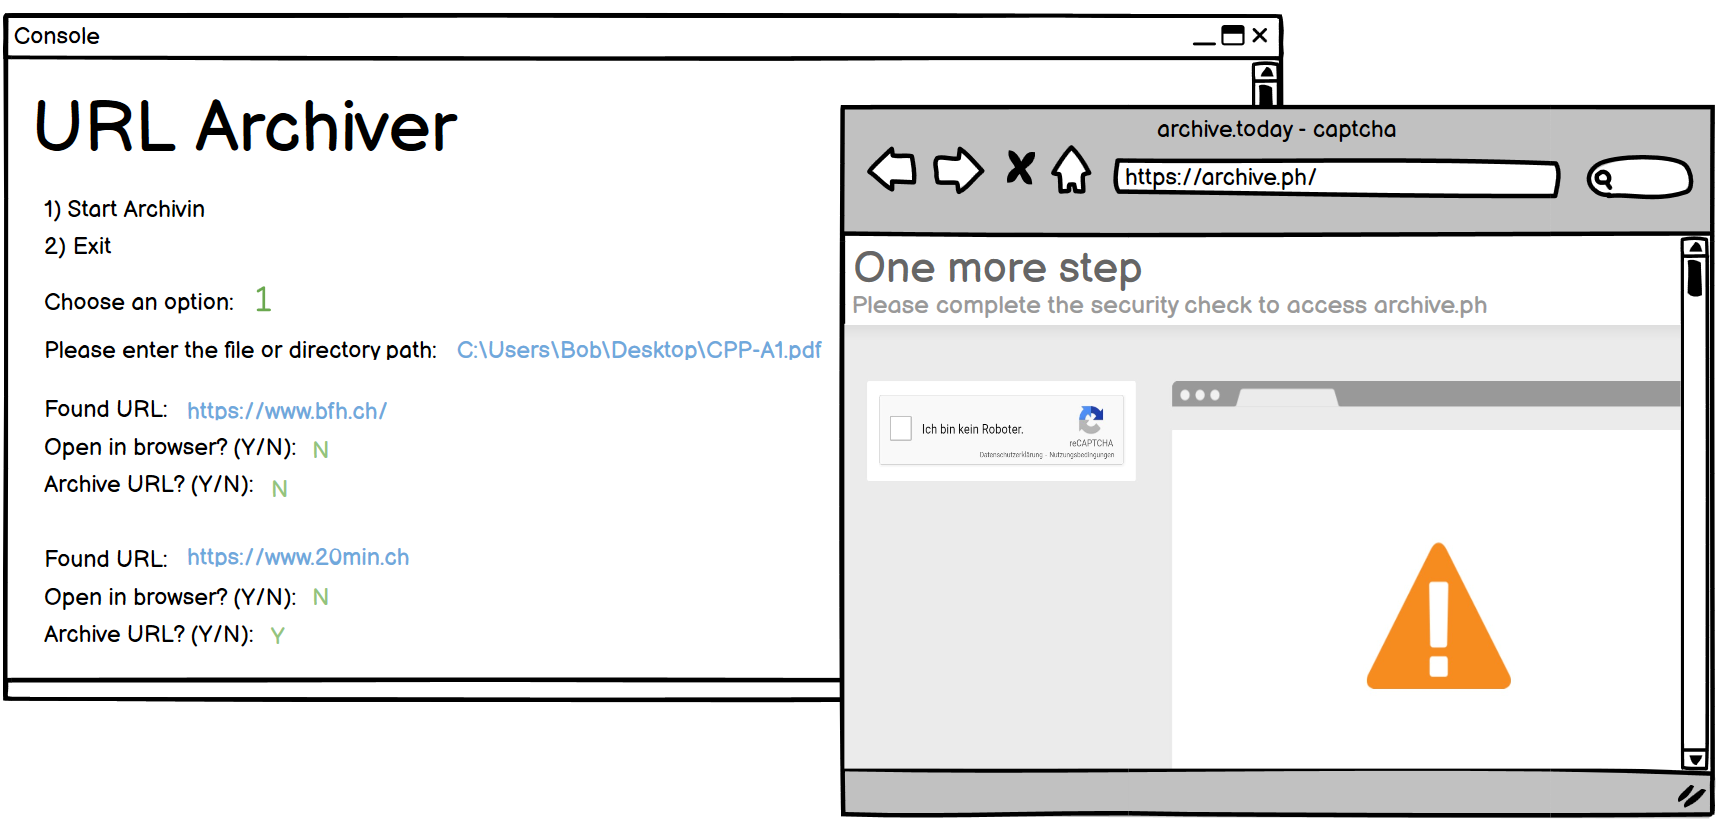
\includegraphics[width=1\textwidth]{pictures/UX-Prototype/Prototype_4}
    \caption{A security step requiring captcha verification to proceed with the archiving process.}
    \label{fig:Archiving_Decision}
\end{figure}
\begin{figure}[h!]
    \centering
    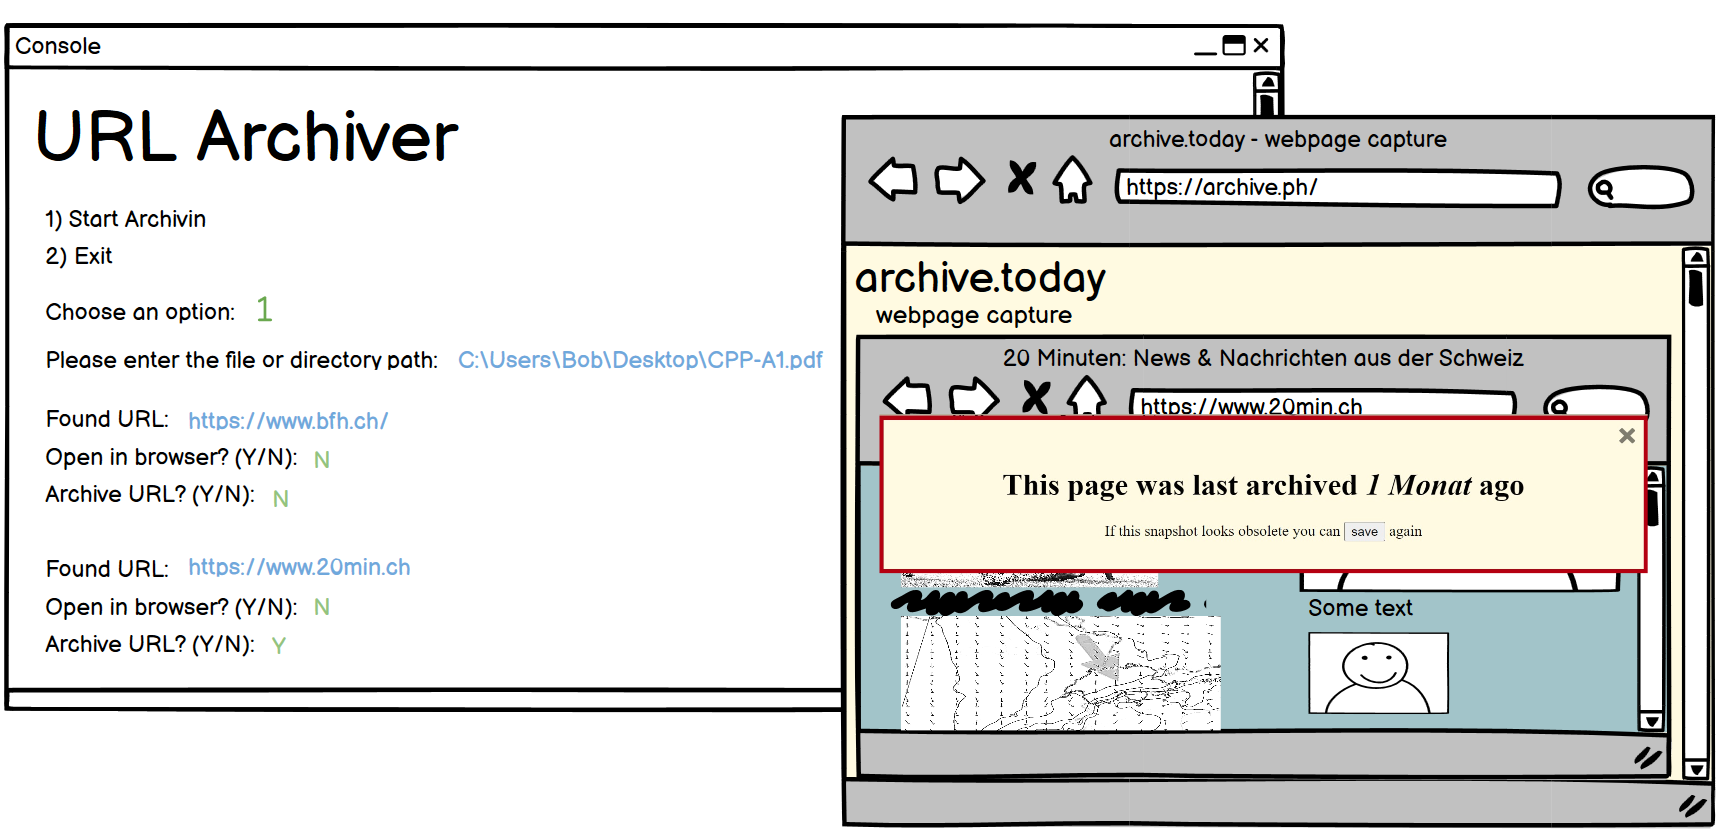
\includegraphics[width=1\textwidth]{pictures/UX-Prototype/Prototype_5}
    \caption{Archive Today informs that the website has been archived before. The application proceeds to re-archive the site.}
    \label{fig:Captcha_Verification}
\end{figure}
\begin{figure}[h!]
    \centering
    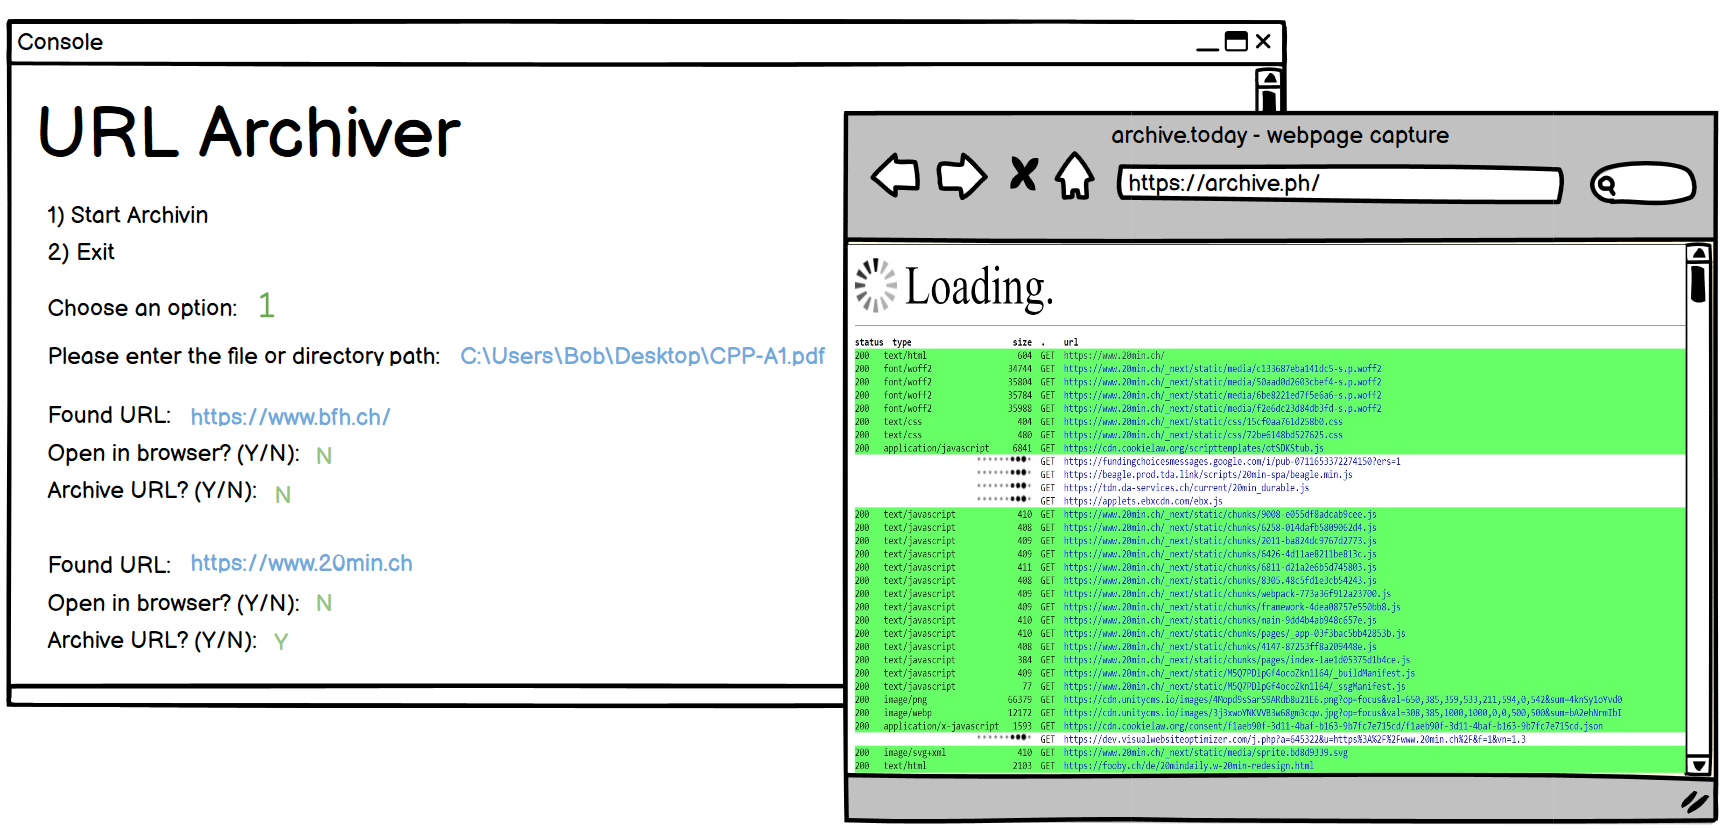
\includegraphics[width=1\textwidth]{pictures/UX-Prototype/Prototype_6}
    \caption{The archiving process is actively underway on the Archive Today platform.}
    \label{fig:Archiving_Confirmation}
\end{figure}
\begin{figure}[h!]
    \centering
    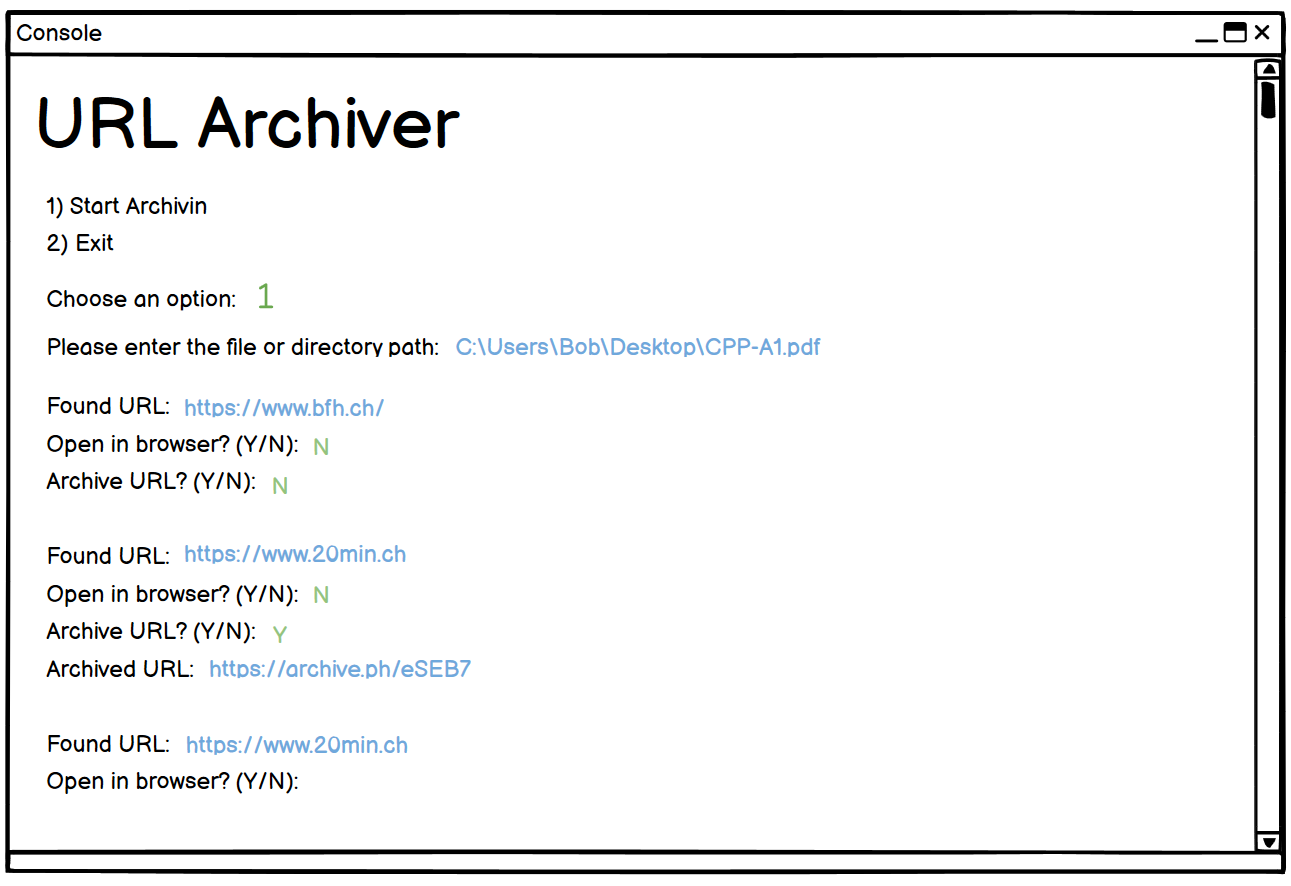
\includegraphics[width=1\textwidth]{pictures/UX-Prototype/Prototype_7}
    \caption{After successful archiving, the system provides the user with a confirmation message and the archived URL.}
    \label{fig:Process_Continuation}
\end{figure}
\clearpage
